% Options for packages loaded elsewhere
\PassOptionsToPackage{unicode}{hyperref}
\PassOptionsToPackage{hyphens}{url}
%
\documentclass[
]{book}
\title{Estadística Aplicada a las Ciencias y la Ingeniería}
\author{Emilio L. Cano}
\date{2021-08-31}

\usepackage{amsmath,amssymb}
\usepackage{lmodern}
\usepackage{iftex}
\ifPDFTeX
  \usepackage[T1]{fontenc}
  \usepackage[utf8]{inputenc}
  \usepackage{textcomp} % provide euro and other symbols
\else % if luatex or xetex
  \usepackage{unicode-math}
  \defaultfontfeatures{Scale=MatchLowercase}
  \defaultfontfeatures[\rmfamily]{Ligatures=TeX,Scale=1}
\fi
% Use upquote if available, for straight quotes in verbatim environments
\IfFileExists{upquote.sty}{\usepackage{upquote}}{}
\IfFileExists{microtype.sty}{% use microtype if available
  \usepackage[]{microtype}
  \UseMicrotypeSet[protrusion]{basicmath} % disable protrusion for tt fonts
}{}
\makeatletter
\@ifundefined{KOMAClassName}{% if non-KOMA class
  \IfFileExists{parskip.sty}{%
    \usepackage{parskip}
  }{% else
    \setlength{\parindent}{0pt}
    \setlength{\parskip}{6pt plus 2pt minus 1pt}}
}{% if KOMA class
  \KOMAoptions{parskip=half}}
\makeatother
\usepackage{xcolor}
\IfFileExists{xurl.sty}{\usepackage{xurl}}{} % add URL line breaks if available
\IfFileExists{bookmark.sty}{\usepackage{bookmark}}{\usepackage{hyperref}}
\hypersetup{
  pdftitle={Estadística Aplicada a las Ciencias y la Ingeniería},
  pdfauthor={Emilio L. Cano},
  hidelinks,
  pdfcreator={LaTeX via pandoc}}
\urlstyle{same} % disable monospaced font for URLs
\usepackage{color}
\usepackage{fancyvrb}
\newcommand{\VerbBar}{|}
\newcommand{\VERB}{\Verb[commandchars=\\\{\}]}
\DefineVerbatimEnvironment{Highlighting}{Verbatim}{commandchars=\\\{\}}
% Add ',fontsize=\small' for more characters per line
\usepackage{framed}
\definecolor{shadecolor}{RGB}{248,248,248}
\newenvironment{Shaded}{\begin{snugshade}}{\end{snugshade}}
\newcommand{\AlertTok}[1]{\textcolor[rgb]{0.94,0.16,0.16}{#1}}
\newcommand{\AnnotationTok}[1]{\textcolor[rgb]{0.56,0.35,0.01}{\textbf{\textit{#1}}}}
\newcommand{\AttributeTok}[1]{\textcolor[rgb]{0.77,0.63,0.00}{#1}}
\newcommand{\BaseNTok}[1]{\textcolor[rgb]{0.00,0.00,0.81}{#1}}
\newcommand{\BuiltInTok}[1]{#1}
\newcommand{\CharTok}[1]{\textcolor[rgb]{0.31,0.60,0.02}{#1}}
\newcommand{\CommentTok}[1]{\textcolor[rgb]{0.56,0.35,0.01}{\textit{#1}}}
\newcommand{\CommentVarTok}[1]{\textcolor[rgb]{0.56,0.35,0.01}{\textbf{\textit{#1}}}}
\newcommand{\ConstantTok}[1]{\textcolor[rgb]{0.00,0.00,0.00}{#1}}
\newcommand{\ControlFlowTok}[1]{\textcolor[rgb]{0.13,0.29,0.53}{\textbf{#1}}}
\newcommand{\DataTypeTok}[1]{\textcolor[rgb]{0.13,0.29,0.53}{#1}}
\newcommand{\DecValTok}[1]{\textcolor[rgb]{0.00,0.00,0.81}{#1}}
\newcommand{\DocumentationTok}[1]{\textcolor[rgb]{0.56,0.35,0.01}{\textbf{\textit{#1}}}}
\newcommand{\ErrorTok}[1]{\textcolor[rgb]{0.64,0.00,0.00}{\textbf{#1}}}
\newcommand{\ExtensionTok}[1]{#1}
\newcommand{\FloatTok}[1]{\textcolor[rgb]{0.00,0.00,0.81}{#1}}
\newcommand{\FunctionTok}[1]{\textcolor[rgb]{0.00,0.00,0.00}{#1}}
\newcommand{\ImportTok}[1]{#1}
\newcommand{\InformationTok}[1]{\textcolor[rgb]{0.56,0.35,0.01}{\textbf{\textit{#1}}}}
\newcommand{\KeywordTok}[1]{\textcolor[rgb]{0.13,0.29,0.53}{\textbf{#1}}}
\newcommand{\NormalTok}[1]{#1}
\newcommand{\OperatorTok}[1]{\textcolor[rgb]{0.81,0.36,0.00}{\textbf{#1}}}
\newcommand{\OtherTok}[1]{\textcolor[rgb]{0.56,0.35,0.01}{#1}}
\newcommand{\PreprocessorTok}[1]{\textcolor[rgb]{0.56,0.35,0.01}{\textit{#1}}}
\newcommand{\RegionMarkerTok}[1]{#1}
\newcommand{\SpecialCharTok}[1]{\textcolor[rgb]{0.00,0.00,0.00}{#1}}
\newcommand{\SpecialStringTok}[1]{\textcolor[rgb]{0.31,0.60,0.02}{#1}}
\newcommand{\StringTok}[1]{\textcolor[rgb]{0.31,0.60,0.02}{#1}}
\newcommand{\VariableTok}[1]{\textcolor[rgb]{0.00,0.00,0.00}{#1}}
\newcommand{\VerbatimStringTok}[1]{\textcolor[rgb]{0.31,0.60,0.02}{#1}}
\newcommand{\WarningTok}[1]{\textcolor[rgb]{0.56,0.35,0.01}{\textbf{\textit{#1}}}}
\usepackage{longtable,booktabs,array}
\usepackage{calc} % for calculating minipage widths
% Correct order of tables after \paragraph or \subparagraph
\usepackage{etoolbox}
\makeatletter
\patchcmd\longtable{\par}{\if@noskipsec\mbox{}\fi\par}{}{}
\makeatother
% Allow footnotes in longtable head/foot
\IfFileExists{footnotehyper.sty}{\usepackage{footnotehyper}}{\usepackage{footnote}}
\makesavenoteenv{longtable}
\usepackage{graphicx}
\makeatletter
\def\maxwidth{\ifdim\Gin@nat@width>\linewidth\linewidth\else\Gin@nat@width\fi}
\def\maxheight{\ifdim\Gin@nat@height>\textheight\textheight\else\Gin@nat@height\fi}
\makeatother
% Scale images if necessary, so that they will not overflow the page
% margins by default, and it is still possible to overwrite the defaults
% using explicit options in \includegraphics[width, height, ...]{}
\setkeys{Gin}{width=\maxwidth,height=\maxheight,keepaspectratio}
% Set default figure placement to htbp
\makeatletter
\def\fps@figure{htbp}
\makeatother
\setlength{\emergencystretch}{3em} % prevent overfull lines
\providecommand{\tightlist}{%
  \setlength{\itemsep}{0pt}\setlength{\parskip}{0pt}}
\setcounter{secnumdepth}{5}
\usepackage{booktabs}
\usepackage[spanish, es-tabla]{babel}

\usepackage{framed,color}
\definecolor{shadecolor}{RGB}{248,248,248}

\newenvironment{rmdejemplo}
  {\begin{rmdblock}{ejemplo}}
  {\end{rmdblock}}
\newenvironment{rmdcafe}
  {\begin{rmdblock}{cafe}}
  {\end{rmdblock}}
\newenvironment{rmdpractica}
  {\begin{rmdblock}{practice}}
  {\end{rmdblock}}
\newenvironment{rmdpremium}
  {\begin{rmdblock}{premium}}
  {\end{rmdblock}}
  
\ifLuaTeX
  \usepackage{selnolig}  % disable illegal ligatures
\fi
\usepackage[]{natbib}
\bibliographystyle{apalike}

\usepackage{amsthm}
\newtheorem{theorem}{Theorem}[chapter]
\newtheorem{lemma}{Lemma}[chapter]
\newtheorem{corollary}{Corollary}[chapter]
\newtheorem{proposition}{Proposition}[chapter]
\newtheorem{conjecture}{Conjecture}[chapter]
\theoremstyle{definition}
\newtheorem{definition}{Definition}[chapter]
\theoremstyle{definition}
\newtheorem{example}{Example}[chapter]
\theoremstyle{definition}
\newtheorem{exercise}{Exercise}[chapter]
\theoremstyle{definition}
\newtheorem{hypothesis}{Hypothesis}[chapter]
\theoremstyle{remark}
\newtheorem*{remark}{Remark}
\newtheorem*{solution}{Solution}
\begin{document}
\maketitle

{
\setcounter{tocdepth}{1}
\tableofcontents
}
\hypertarget{prefacio}{%
\chapter*{Prefacio}\label{prefacio}}
\addcontentsline{toc}{chapter}{Prefacio}

Este libro incluye los contenidos habitualmente presentes en el currículo
de asignaturas de \textbf{Estadística} de los grados Ciencias e Ingenierías de universidades españolas.
Si bien existe abundante material bibliográfico
que cubre los contenidos de estas asignaturas, quería elaborar un material
propio que no fuera solamente para mis clases sino algo más
\emph{global}. Por otra parte, me motiva cubrir el hueco de los materiales
de acceso gratuito con la opción de comprar una edición
impresa\footnote{A la espera de encontrar editorial.} y con el enfoque
que se menciona en el siguiente apartado. Por otra parte, los libros publicados
originalmente en inglés y traducidos al español a menudo me resultan lejanos
a nuestro idioma (por muy buenas que sean las traducciones, los ejemplos en \emph{acres}
no son muy intuitivos para un lector español). Espero que también sirva para
lectores de otros países de habla hispana.

\hypertarget{estuxe1ndares-y-software}{%
\section*{Estándares y software}\label{estuxe1ndares-y-software}}
\addcontentsline{toc}{section}{Estándares y software}

Los contenidos de este libro se basan en dos paradigmas que están presentes
en los intereses de investigación y docencia del autor: los \textbf{estándares} y
el \textbf{software libre}. En lo que se refiere a estándares, la notación utilizada,
definiciones y fórmulas se ajustarán el máximo posible a la utilizada en normas
nacionales e internacionales sobre metodología estadística. Estas normas se
citarán pertinentemente a lo largo del texto. En cuanto al software libre,
se proporcionarán instrucciones para resolver los ejemplos
que ilustran la teoría utilizando software libre.
No obstante, el uso del software es
auxiliar al texto y se puede seguir sin necesidad de utilizar
los programas. Según lo que proceda en cada caso, se utilizará
software de hoja de cálculo, el software estadístico y lenguaje de
programación
\textbf{R} \citep{R-base},
y el software de álgebra computacional \textbf{Máxima}\footnote{\url{http://maxima.sourceforge.net/es/}}.
Respecto al software de hoja de cálculo, las fórmulas utilizadas se han probado
en el software libre \textbf{LibreOffice}\footnote{\url{https://es.libreoffice.org}}, en \textbf{Hojas de Cálculo de Google}\footnote{\url{https://www.google.es/intl/es/sheets/about/}} y
también en \textbf{Microsoft EXCEL}\footnote{\url{https://products.office.com/es-es/excel}} que,
aunque no es software libre, su uso
está más que generalizado y normalmente los estudiantes disponen de licencia de uso
a través de su universidad. En caso de que el nombre de la función sea distinta
en EXCEL, se indicará en el propio ejemplo.

Las normas son clave para el desarrollo económico de un país. Estudios en diversos países,
incluido España, han demostrado que la aportación de la normalización a su economía es del 1\% del PIB\footnote{\url{http://www.aenor.es/DescargasWeb/normas/como-beneficia-es.pdf}}. La
Asociación Española de Normalización (UNE) es el organismo legalmente
responsable del desarrollo y difusión de las normas técnicas en España.
Además, representa a España en los organismos internacionales de normalización como
\href{https://www.iso.org/}{ISO}\footnote{\url{https://www.iso.org/}} y \href{https://www.cen.eu/}{CEN}\footnote{\url{https://www.cen.eu/}}.

Las normas sobre estadística que surgen de ISO las elabora el \emph{Technical Committee}
ISO TC 69\footnote{\url{https://www.iso.org/committee/49742/x/catalogue/}} \emph{Statistical Methods}.
Por su parte, el subcomité técnico de normalización
CTN 66/SC 3\footnote{\url{https://www.une.org/encuentra-tu-norma/comites-tecnicos-de-normalizacion/comite/?c=CTN\%2066/SC\%203}}, Métodos Estadísticos,
participa como miembro nacional en ese comité ISO.
Las normas que son de interés en España, se ratifican en inglés o se traducen
al español como normas UNE. Para una descripción más completa de la elaboración
de normas, véase \citet{cano2015qcr}.

Este libro se ha elaborado utilizando el lenguaje \emph{Markdown} con el propio
software \textbf{R} y el paquete \textbf{bookdown} \citep{R-bookdown}.
Se incluyen una gran cantidad de ejemplos resueltos tanto de forma analítica
como mediante software. En algunos casos se proporciona el uso de funciones
en hojas de cálculo (y el resultado obtenido con un recuadro).
En otros, código de R, que aparecen en el texto
sombreados y con la sintaxis coloreada, como el fragmento a continuación
donde se puede comprobar la sesión de R en la que ha sido generado este material.
Obsérvese que los resultados se muestran precedidos de los símbolos
\texttt{\#\textgreater{}}.

\begin{Shaded}
\begin{Highlighting}[]
\FunctionTok{sessionInfo}\NormalTok{()}
\CommentTok{\#\textgreater{} R version 4.1.1 (2021{-}08{-}10)}
\CommentTok{\#\textgreater{} Platform: x86\_64{-}apple{-}darwin17.0 (64{-}bit)}
\CommentTok{\#\textgreater{} Running under: macOS Big Sur 10.16}
\CommentTok{\#\textgreater{} }
\CommentTok{\#\textgreater{} Matrix products: default}
\CommentTok{\#\textgreater{} BLAS:   /Library/Frameworks/R.framework/Versions/4.1/Resources/lib/libRblas.0.dylib}
\CommentTok{\#\textgreater{} LAPACK: /Library/Frameworks/R.framework/Versions/4.1/Resources/lib/libRlapack.dylib}
\CommentTok{\#\textgreater{} }
\CommentTok{\#\textgreater{} locale:}
\CommentTok{\#\textgreater{} [1] es\_ES.UTF{-}8/es\_ES.UTF{-}8/es\_ES.UTF{-}8/C/es\_ES.UTF{-}8/es\_ES.UTF{-}8}
\CommentTok{\#\textgreater{} }
\CommentTok{\#\textgreater{} attached base packages:}
\CommentTok{\#\textgreater{} [1] stats     graphics  grDevices utils     datasets }
\CommentTok{\#\textgreater{} [6] methods   base     }
\CommentTok{\#\textgreater{} }
\CommentTok{\#\textgreater{} loaded via a namespace (and not attached):}
\CommentTok{\#\textgreater{}  [1] compiler\_4.1.1  magrittr\_2.0.1  fastmap\_1.1.0  }
\CommentTok{\#\textgreater{}  [4] bookdown\_0.23.4 htmltools\_0.5.2 tools\_4.1.1    }
\CommentTok{\#\textgreater{}  [7] yaml\_2.2.1      stringi\_1.7.4   rmarkdown\_2.10 }
\CommentTok{\#\textgreater{} [10] knitr\_1.33      stringr\_1.4.0   digest\_0.6.27  }
\CommentTok{\#\textgreater{} [13] xfun\_0.25       rlang\_0.4.11    evaluate\_0.14}
\end{Highlighting}
\end{Shaded}

Normalmente, la descripción o enunciado de los ejemplos se incluyen en bloques
con el siguiente aspecto:

Esto es un ejemplo. A continuación puede mostrarse código o no.

Cuando el ejemplo incluya explicaciones sobre cómo resolverlo con software,
estas explicaciones aparecerán en bloques con el siguiente aspecto:

\textbf{HOJA DE CÁLCULO}

La función \texttt{FACT} obtiene el factorial de un número x (\(x!\)):

\texttt{=FACT(5)}
\(\boxed{\mathsf{120}}\)

También se incluirán con el formato anterior indicaciones para usar la calculadora
científica, cuando esto sea posible.
El texto incluye otros bloques con información de distinto tipo.

Este contenido se considera avanzado. El lector principiante puede saltarse estos apartados
y volver sobre ellos en una segunda lectura.

Estos bloques están pensados para incluir información curiosa o complementaria
para poner en contexto las explicaciones.

\hypertarget{sobre-el-autor}{%
\section*{Sobre el autor}\label{sobre-el-autor}}
\addcontentsline{toc}{section}{Sobre el autor}

Actualmente soy Profesor Ayudante Doctor en la Escuela Técnica Superior de Ingeniería Informática e investigador en el Data Science Laboratory de la Universidad Rey Juan Carlos. Sus intereses de investigación incluyen Estadística Aplicada, Aprendizaje Estadístico y Metodologías pra la Calidad. afiliaciones. Previamente ha sido profesor en la Universidad de Castilla-La Mancha, donde sigue colaborando en docencia e investigación, y Estadístico en empresas del sector privado de diversos sectores.

Presidente del subcomité técnico de normalización UNE (miembro de ISO) CTN 66/SC 3 (Métodos Estadísticos). Profesor en la Asociación Española para la Calidad (AEC). Presidente de la asociación ``Comunidad R Hispano''.

Más sobre mí, información actualizada y publicaciones: \url{https://emilio.lcano.com}.\\
Contacto: \href{mailto:emilio@lcano.com}{\nolinkurl{emilio@lcano.com}}

El material se proporciona bajo licencia CC-BY-NC-ND.
Todos los logotipos y marcas comerciales que puedan aparecer en este texto
son propiedad de sus respectivos dueños y se incluyen en este texto únicamente
con fines formativos. Se ha puesto especial cuidado en la adecuada atribución
del material no elaborado por el autor, véase el Apéndice \ref{creditos}.
Aún así, si detecta algún uso
indebido de material protegido póngase en contacto con el autor y será retirado.
Igualmente, contacte con el autor \textbf{si desea utilizar este material con fines
comerciales}.


\includegraphics[width=1.22in]{images/by-nc-nd}

Este obra está bajo una licencia de Creative Commons Reconocimiento-NoComercial-SinObraDerivada 4.0 Internacional.

\hypertarget{agradecimientos}{%
\section*{Agradecimientos}\label{agradecimientos}}
\addcontentsline{toc}{section}{Agradecimientos}

Este libro es el resultado de años de trabajo en la docencia, investigación
y transferencia de conocimiento en el campo de la Estadística. Está construido
a partir de las contribuciones a lo largo de los años de compañeros y amigos
como Javier M. Moguerza, Andrés Redchuk, Felipe Ortega, Mariano Prieto,
Miguel Ángel Tarancón, Víctor M. Casero, Matías Gámez, y muchos otros (perdón
a \href{mailto:l@s}{\nolinkurl{l@s}} \href{mailto:omitid@s}{\nolinkurl{omitid@s}} por no ser más exhaustivo).

Especial agradecimiento a toda la comunidad del software libre y
lenguaje de programación R, y en especial al R Core Team y al equipo
de RStudio.

\hypertarget{hello-bookdown}{%
\chapter{Hello bookdown}\label{hello-bookdown}}

All chapters start with a first-level heading followed by your chapter title, like the line above. There should be only one first-level heading (\texttt{\#}) per .Rmd file.

\hypertarget{a-section}{%
\section{A section}\label{a-section}}

All chapter sections start with a second-level (\texttt{\#\#}) or higher heading followed by your section title, like the sections above and below here. You can have as many as you want within a chapter.

\hypertarget{an-unnumbered-section}{%
\subsection*{An unnumbered section}\label{an-unnumbered-section}}
\addcontentsline{toc}{subsection}{An unnumbered section}

Chapters and sections are numbered by default. To un-number a heading, add a \texttt{\{.unnumbered\}} or the shorter \texttt{\{-\}} at the end of the heading, like in this section.

\hypertarget{cross}{%
\chapter{Cross-references}\label{cross}}

Cross-references make it easier for your readers to find and link to elements in your book.

\hypertarget{chapters-and-sub-chapters}{%
\section{Chapters and sub-chapters}\label{chapters-and-sub-chapters}}

There are two steps to cross-reference any heading:

\begin{enumerate}
\def\labelenumi{\arabic{enumi}.}
\tightlist
\item
  Label the heading: \texttt{\#\ Hello\ world\ \{\#nice-label\}}.

  \begin{itemize}
  \tightlist
  \item
    Leave the label off if you like the automated heading generated based on your heading title: for example, \texttt{\#\ Hello\ world} = \texttt{\#\ Hello\ world\ \{\#hello-world\}}.
  \item
    To label an un-numbered heading, use: \texttt{\#\ Hello\ world\ \{-\#nice-label\}} or \texttt{\{\#\ Hello\ world\ .unnumbered\}}.
  \end{itemize}
\item
  Next, reference the labeled heading anywhere in the text using \texttt{\textbackslash{}@ref(nice-label)}; for example, please see Chapter \ref{cross}.

  \begin{itemize}
  \tightlist
  \item
    If you prefer text as the link instead of a numbered reference use: \protect\hyperlink{cross}{any text you want can go here}.
  \end{itemize}
\end{enumerate}

\hypertarget{captioned-figures-and-tables}{%
\section{Captioned figures and tables}\label{captioned-figures-and-tables}}

Figures and tables \emph{with captions} can also be cross-referenced from elsewhere in your book using \texttt{\textbackslash{}@ref(fig:chunk-label)} and \texttt{\textbackslash{}@ref(tab:chunk-label)}, respectively.

See Figure \ref{fig:nice-fig}.

\begin{Shaded}
\begin{Highlighting}[]
\FunctionTok{par}\NormalTok{(}\AttributeTok{mar =} \FunctionTok{c}\NormalTok{(}\DecValTok{4}\NormalTok{, }\DecValTok{4}\NormalTok{, .}\DecValTok{1}\NormalTok{, .}\DecValTok{1}\NormalTok{))}
\FunctionTok{plot}\NormalTok{(pressure, }\AttributeTok{type =} \StringTok{\textquotesingle{}b\textquotesingle{}}\NormalTok{, }\AttributeTok{pch =} \DecValTok{19}\NormalTok{)}
\end{Highlighting}
\end{Shaded}

\begin{figure}

{\centering 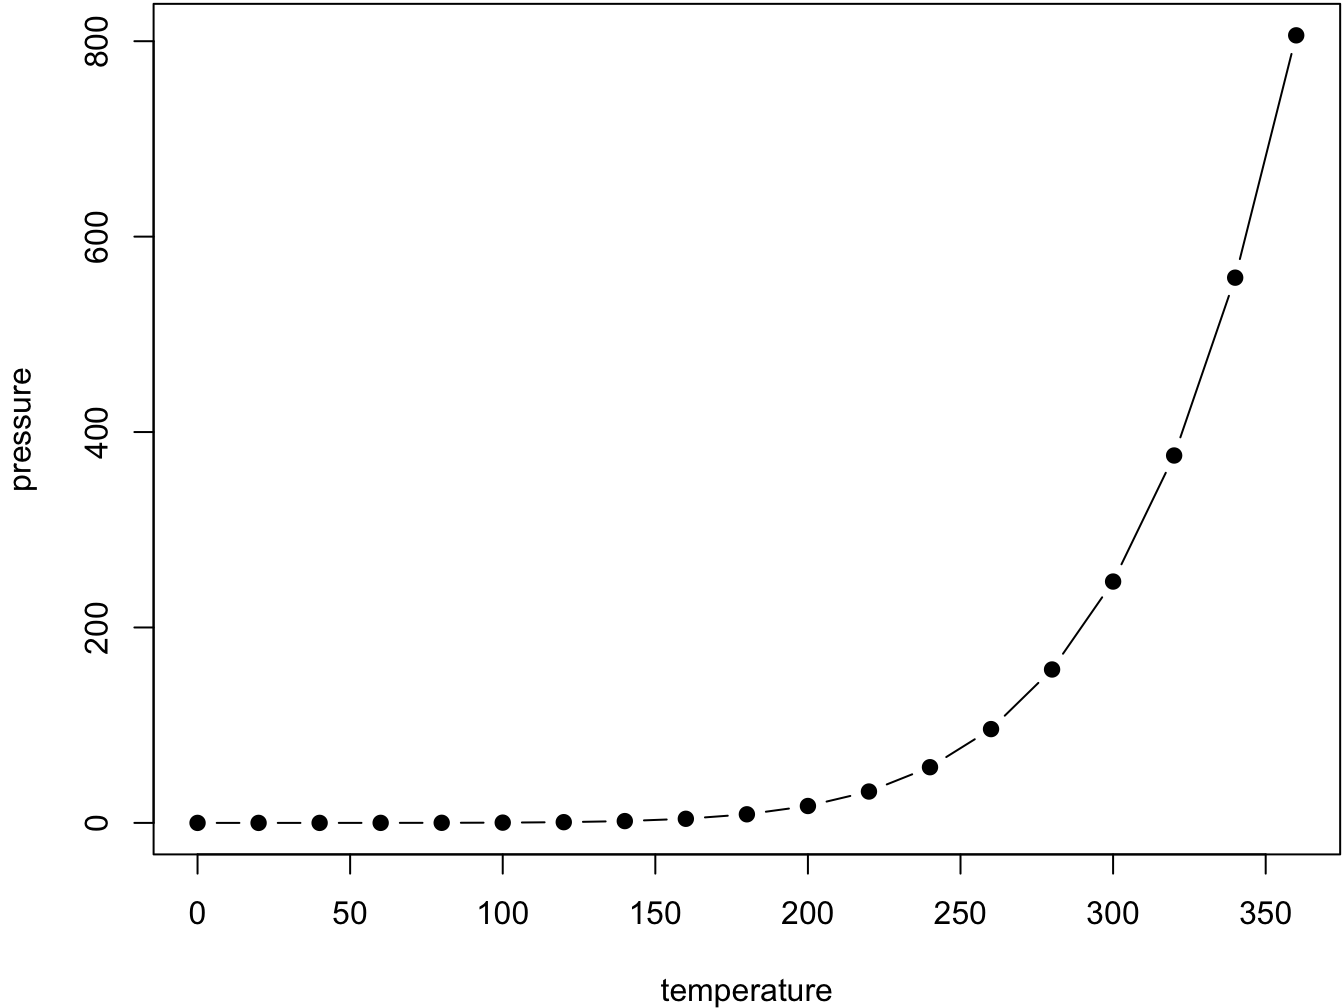
\includegraphics[width=0.8\linewidth]{02-cross-refs_files/figure-latex/nice-fig-1} 

}

\caption{Here is a nice figure!}\label{fig:nice-fig}
\end{figure}

Don't miss Table \ref{tab:nice-tab}.

\begin{Shaded}
\begin{Highlighting}[]
\NormalTok{knitr}\SpecialCharTok{::}\FunctionTok{kable}\NormalTok{(}
  \FunctionTok{head}\NormalTok{(pressure, }\DecValTok{10}\NormalTok{), }\AttributeTok{caption =} \StringTok{\textquotesingle{}Here is a nice table!\textquotesingle{}}\NormalTok{,}
  \AttributeTok{booktabs =} \ConstantTok{TRUE}
\NormalTok{)}
\end{Highlighting}
\end{Shaded}

\begin{table}

\caption{\label{tab:nice-tab}Here is a nice table!}
\centering
\begin{tabular}[t]{rr}
\toprule
temperature & pressure\\
\midrule
0 & 0.0002\\
20 & 0.0012\\
40 & 0.0060\\
60 & 0.0300\\
80 & 0.0900\\
\addlinespace
100 & 0.2700\\
120 & 0.7500\\
140 & 1.8500\\
160 & 4.2000\\
180 & 8.8000\\
\bottomrule
\end{tabular}
\end{table}

\hypertarget{parts}{%
\chapter{Parts}\label{parts}}

You can add parts to organize one or more book chapters together. Parts can be inserted at the top of an .Rmd file, before the first-level chapter heading in that same file.

Add a numbered part: \texttt{\#\ (PART)\ Act\ one\ \{-\}} (followed by \texttt{\#\ A\ chapter})

Add an unnumbered part: \texttt{\#\ (PART\textbackslash{}*)\ Act\ one\ \{-\}} (followed by \texttt{\#\ A\ chapter})

Add an appendix as a special kind of un-numbered part: \texttt{\#\ (APPENDIX)\ Other\ stuff\ \{-\}} (followed by \texttt{\#\ A\ chapter}). Chapters in an appendix are prepended with letters instead of numbers.

\hypertarget{footnotes-and-citations}{%
\chapter{Footnotes and citations}\label{footnotes-and-citations}}

\hypertarget{footnotes}{%
\section{Footnotes}\label{footnotes}}

Footnotes are put inside the square brackets after a caret \texttt{\^{}{[}{]}}. Like this one \footnote{This is a footnote.}.

\hypertarget{citations}{%
\section{Citations}\label{citations}}

Reference items in your bibliography file(s) using \texttt{@key}.

For example, we are using the \textbf{bookdown} package \citep{R-bookdown} (check out the last code chunk in index.Rmd to see how this citation key was added) in this sample book, which was built on top of R Markdown and \textbf{knitr} \citep{xie2015} (this citation was added manually in an external file book.bib).
Note that the \texttt{.bib} files need to be listed in the index.Rmd with the YAML \texttt{bibliography} key.

The \texttt{bs4\_book} theme makes footnotes appear inline when you click on them. In this example book, we added \texttt{csl:\ chicago-fullnote-bibliography.csl} to the \texttt{index.Rmd} YAML, and include the \texttt{.csl} file. To download a new style, we recommend: \url{https://www.zotero.org/styles/}

The RStudio Visual Markdown Editor can also make it easier to insert citations: \url{https://rstudio.github.io/visual-markdown-editing/\#/citations}

\hypertarget{blocks}{%
\chapter{Blocks}\label{blocks}}

\hypertarget{equations}{%
\section{Equations}\label{equations}}

Here is an equation.

\begin{equation} 
  f\left(k\right) = \binom{n}{k} p^k\left(1-p\right)^{n-k}
  \label{eq:binom}
\end{equation}

You may refer to using \texttt{\textbackslash{}@ref(eq:binom)}, like see Equation \eqref{eq:binom}.

\hypertarget{theorems-and-proofs}{%
\section{Theorems and proofs}\label{theorems-and-proofs}}

Labeled theorems can be referenced in text using \texttt{\textbackslash{}@ref(thm:tri)}, for example, check out this smart theorem \ref{thm:tri}.

\begin{theorem}
\protect\hypertarget{thm:tri}{}\label{thm:tri}For a right triangle, if \(c\) denotes the \emph{length} of the hypotenuse
and \(a\) and \(b\) denote the lengths of the \textbf{other} two sides, we have
\[a^2 + b^2 = c^2\]
\end{theorem}

Read more here \url{https://bookdown.org/yihui/bookdown/markdown-extensions-by-bookdown.html}.

\hypertarget{callout-blocks}{%
\section{Callout blocks}\label{callout-blocks}}

The \texttt{bs4\_book} theme also includes special callout blocks, like this \texttt{.rmdnote}.

You can use \textbf{markdown} inside a block.

\begin{Shaded}
\begin{Highlighting}[]
\FunctionTok{head}\NormalTok{(beaver1, }\AttributeTok{n =} \DecValTok{5}\NormalTok{)}
\CommentTok{\#\textgreater{}   day time  temp activ}
\CommentTok{\#\textgreater{} 1 346  840 36.33     0}
\CommentTok{\#\textgreater{} 2 346  850 36.34     0}
\CommentTok{\#\textgreater{} 3 346  900 36.35     0}
\CommentTok{\#\textgreater{} 4 346  910 36.42     0}
\CommentTok{\#\textgreater{} 5 346  920 36.55     0}
\end{Highlighting}
\end{Shaded}

It is up to the user to define the appearance of these blocks for LaTeX output.

You may also use: \texttt{.rmdcaution}, \texttt{.rmdimportant}, \texttt{.rmdtip}, or \texttt{.rmdwarning} as the block name.

The R Markdown Cookbook provides more help on how to use custom blocks to design your own callouts: \url{https://bookdown.org/yihui/rmarkdown-cookbook/custom-blocks.html}

\hypertarget{sharing-your-book}{%
\chapter{Sharing your book}\label{sharing-your-book}}

\hypertarget{publishing}{%
\section{Publishing}\label{publishing}}

HTML books can be published online, see: \url{https://bookdown.org/yihui/bookdown/publishing.html}

\hypertarget{pages}{%
\section{404 pages}\label{pages}}

By default, users will be directed to a 404 page if they try to access a webpage that cannot be found. If you'd like to customize your 404 page instead of using the default, you may add either a \texttt{\_404.Rmd} or \texttt{\_404.md} file to your project root and use code and/or Markdown syntax.

\hypertarget{metadata-for-sharing}{%
\section{Metadata for sharing}\label{metadata-for-sharing}}

Bookdown HTML books will provide HTML metadata for social sharing on platforms like Twitter, Facebook, and LinkedIn, using information you provide in the \texttt{index.Rmd} YAML. To setup, set the \texttt{url} for your book and the path to your \texttt{cover-image} file. Your book's \texttt{title} and \texttt{description} are also used.

This \texttt{bs4\_book} provides enhanced metadata for social sharing, so that each chapter shared will have a unique description, auto-generated based on the content.

Specify your book's source repository on GitHub as the \texttt{repo} in the \texttt{\_output.yml} file, which allows users to view each chapter's source file or suggest an edit. Read more about the features of this output format here:

\url{https://pkgs.rstudio.com/bookdown/reference/bs4_book.html}

Or use:

\begin{Shaded}
\begin{Highlighting}[]
\NormalTok{?bookdown}\SpecialCharTok{::}\NormalTok{bs4\_book}
\end{Highlighting}
\end{Shaded}


  \bibliography{book.bib,packages.bib}

\end{document}
